%%%%%%%%%%%%%%%%%%%%%%%%%%%%%%%%%%%%%%%%%%%%%%%%%%%%%%%%%%%%%%%%%
%                                                               %
%                       Legal Notice                            %
%                                                               %
% This document is copyright (C) Jason Gobat & Darren Atkinson	%
%                                                               %
%%%%%%%%%%%%%%%%%%%%%%%%%%%%%%%%%%%%%%%%%%%%%%%%%%%%%%%%%%%%%%%%%

\newpage{\pagestyle{empty}\cleardoublepage}

\chapter{The \felt{} Element Library}
\label{elements}

\section{Introduction}
\label{elements.intro}

The \felt{} element library contains line, plane and solid elements.
Line elements include a one-dimensional spring ({\tt spring}), a bar or truss 
element ({\tt truss}), two- and 
three-dimensional Euler-Bernoulli beams ({\tt beam} and {\tt beam3d}), and
a two-dimensional beam based on Timoshenko theory, ({\tt timoshenko}). The
set of planar elements consists of constant strain triangles  
({\tt CSTPlaneStrain} and {\tt CSTPlaneStress}), isoparametric quadrilaterals 
({\tt iso2d\_PlaneStress}, {\tt iso2d\_PlaneStrain}, {\tt quad\_PlaneStrain}, 
{\tt quad\_PlaneStress}) and an HTK plate bending element ({\tt htk}).
The only solid element in the library is an eight node brick ({\tt brick}).
There is an axisymmetric triangular element ({\tt axisymmetric}).
The only elements available for thermal analysis are a simple one-dimensional
line element ({\tt rod}) and a constrant temperature gradient triangular
element ({\tt ctg}).  In the above list, the names in parentheses indicate 
the actual symbolic type names of the elements.

The number of 
nodes and the material properties needed for defining each element and the DOF 
that the element affects are summarized in the table below.  A brief 
description for each element follows the table; detailed derivations of element 
stiffness matrices can be found in any number of finite element textbooks.
\begin{table}
\begin{center}
\small{
 \begin{tabular}{|l|c|l|l|}
  \hline
  Element type name	& nodes	& Material properties 	& DOFs	\\
  \hline\hline
  \tt truss		 & 2	& \tt E,A,(rho)		& \tt Tx,Ty,Tz \\
  \tt spring             & 2    & \tt E,A,(rho)         & \tt Tx \\
  \tt beam		 & 2	& \tt E,A,Ix,(rho)	& \tt Tx,Ty,Rz \\
  \tt beam3d		 & 2	& \tt E,A,Iy,Iz,J,G,(rho) & \tt Tx,Ty,Tz,Rx,Ry,Rz \\
  \tt timoshenko         & 2    & \tt E,A,Ix,G,kappa,(rho)& \tt Tx,Ty,Rz \\
  \tt CSTPlaneStress	 & 3	& \tt E,t,nu,(rho)	& \tt Tx,Ty \\
  \tt CSTPlaneStrain	 & 3	& \tt E,t,nu,(rho)	& \tt Tx,Ty \\
  \tt quad\_PlaneStress	 & 4	& \tt E,t,nu,(rho)	& \tt Tx,Ty \\
  \tt quad\_PlaneStrain	 & 4	& \tt E,t,nu,(rho)	& \tt Tx,Ty \\
  \tt iso2d\_PlaneStress & 9	& \tt E,t,nu,(rho)	& \tt Tx,Ty \\
  \tt iso2d\_PlaneStrain & 9	& \tt E,t,nu,(rho)	& \tt Tx,Ty \\
  \tt htk                & 4    & \tt E,t,nu,kappa,(rho) & \tt Tz,Rx,Ry \\
  \tt brick              & 8    & \tt E,nu,(rho)	& \tt Tx,Ty,Tz \\
  \tt axisymmetric       & 3    & \tt E,nu,(rho)        & \tt Tx, Ty \\ 
  \tt rod		 & 2 	& \tt A,Kx,(c,rho)	& \tt Tx \\
  \tt ctg		 & 3	& \tt t,Kx,Ky,(c,rho)	& \tt Tx \\
  \hline
 \end{tabular}
}
\end{center}
\caption[Description of the materials required for and local DOF affected
         by the various element types.]
        {Description of the materials required for and local DOF affected
         by the various element types.  The material properties in ()
         indicate properties that are only required during a non-static
         analysis.}
\end{table}

\section{Structural analysis elements}

\subsection{Truss and spring elements}
\label{elements.truss}

Truss or bar elements are the simplest type of element in the library.  They 
are two-node, three-dimensional linear elements which are assumed to deform in 
the axial direction only.  They might find application in a simple bridge 
simulation (the classic example of truss elements) or as springs (as in the 
above example where the spring stiffness, $k$, is given by $EA/L$ of the truss 
element).  The truss element in the \felt{} library uses the classical linear 
shape functions, $N_1 = x/L$ and $N_2 = 1 - x/L$.  Any introductory text on finite 
element analysis (for mechanics at least) probably starts out by deriving the 
stiffness matrix for just such an element; see Chapter 3 of \cite{logan:fem} for 
instance.  The stiffness matrix for this type of element in 
the local element two-dimensional reference frame is the familiar
\begin{equation}
{\hat k}=\left[\matrix{
EA/L	& -EA/L \cr
-EA/L	& EA/L \cr
}\right].
\end{equation}
The lumped mass formulation of the local mass matrix is given by 
\begin{equation}
{\hat m}_{l} = {\rho A L \over 2} \left[\matrix{
1 & 0 \cr
0 & 1 \cr
}\right],
\end{equation}
and the consistent mass formulation by
\begin{equation}
{\hat m}_{c} ={\rho A L \over 6} \left[\matrix{
2 & 1 \cr
1 & 2 \cr
}\right].
\end{equation}

The $2 \times 2$ matrices in local element coordinates are transformed
into the global coordinate system (and into $6 \times 6$ form) according to 
\begin{equation}
k = T^{\rm T} {\hat k} T,
\label{transform}
\end{equation}
where the transformation matrix is given by
\begin{equation}
T = \left[\matrix{
\cos{\theta_x} & \cos{\theta_y} & \cos{\theta_z} & 0 & 0 & 0 \cr
0 & 0 & 0 & \cos{\theta_x} & \cos{\theta_y} & \cos{\theta_z} \cr
}
\right].
\end{equation}
The direction cosines are simply the projections of the local coodinate axes
onto the global coordinate axes,
\begin{eqnarray}
\label{cos_theta_x}
\cos{\theta_{x}} = {{x_{1} - x_{2}} \over L}, \\
\label{cos_theta_y}
\cos{\theta_{y}} = {{y_{1} - y_{2}} \over L}, \\
\cos{\theta_{z}} = {{z_{1} - z_{2}} \over L}.
\end{eqnarray}

The stress calculated for truss elements is the axial stress (not load).  
A positive quantity indicates tension, negative indicates compression.  
If a distributed load is assigned to a truss element it is assumed to be a 
linearly distributed axial loading condition (i.e., it must be directed
{\tt parallel}).  Nothing else makes much sense 
since a truss element cannot carry bending or shear forces along its length.  
The sign convention for the magnitude of the load pairs is positive for loads 
pointing from local node 1 to local node 2.

The spring element included in \felt{} is simply the truss element described
above without the transformation from local element coordinates to global
coordinates.  What this means is that the element matrices are only
$2 \times 2$ and because of this they must be defined only along the global
x-axis.  Distributed loads are not supported by spring elements.

\subsection{Euler-Bernoulli beam elements}
\label{elements.beam}

\subsubsection{Special case two-dimensional element}

A beam element is a two-dimensional, two-node linear element which can carry 
in-plane axial, shear and bending forces.  The moment of inertia used in 
stiffness calculations (specified with {\tt Ix}) is the bending moment 
of inertia 
about the cross-section x-x axis (which in global coordinates is bending 
about the z-axis).  Like the truss element described above, the beam element 
in the \felt{} library is also a standard in many textbooks; the following
stiffness matrix should also look relatively familiar,
\begin{equation}
{\hat k}=\left[\matrix{
AE/L	& 0	    & 0		& -AE/L		& 0		& 0        \cr
0	& 12EI/L^3  & 6EI/L^2	& 0		& -12EI/L^3	& 6EI/L^2  \cr
0	& 6EI/L^2   & 4EI/L	& 0		& -6EI/L^2	& 2EI/L    \cr
-AE/L	& 0	    & 0		& AE/L 		& 0		& 0        \cr
0	& -12EI/L^3 & -6EI/L^2	& 0		& 12EI/L^3	& -6EI/L^2 \cr
0	& 6EI/L^2   & 2EI/L	& 0		& -6EI/L^2	& 4EI/L    \cr
}\right].
\end{equation}
The lumped mass matrix for the beam element is defined as 
\begin{equation}
\label{beam_lumped}
{\hat m}_{l}={\rho A L \over 2} \left[\matrix{
1 & 0 & 0 & 0 & 0 & 0 \cr
0 & 1 & 0 & 0 & 0 & 0 \cr
0 & 0 & {L^{2} \over 12} & 0 & 0 & 0 \cr
0 & 0 & 0 & 1 & 0 & 0 \cr
0 & 0 & 0 & 0 & 1 & 0 \cr
0 & 0 & 0 & 0 & 0 & {L^{2} \over 12} \cr
}\right],
\end{equation}
and the consistent mass matrix as
\begin{equation}
{\hat m}_{c}={\rho A L \over 420} \left[\matrix{
140 & 0    & 0     & 70  & 0    & 0     \cr
0   & 156  & 22L   & 0   & 54   & -13L  \cr
0   & 22L  & 4L^2  & 0   & 13L  & -3L^2 \cr
70  & 0    & 0     & 140 & 0    & 0     \cr
0   & 54   & 13L   & 0   & 156  & -22L  \cr
0   & -13L & -3L^2 & 0   & -22L & 4L^2  \cr
}\right].
\end{equation}
The basis for these mass matrices should also be readily available in many 
textbooks.  The transformation from local element coordinates into 
global coordinates is of the same form as equation~\ref{transform}; the
actual transform matrix for two-dimensional beams is given by
\begin{equation}
T = \left[\matrix{
\cos{\theta_x} & \cos{\theta_y} & 0 & 0 & 0 & 0 \cr
-\cos{\theta_y} & \cos{\theta_x} & 0 & 0 & 0 & 0 \cr
0 & 0 & 1 & 0 & 0 & 0 \cr
0 & 0 & 0 & \cos{\theta_x} & \cos{\theta_y} & 0 \cr
0 & 0 & 0 & -\cos{\theta_y} & \cos{\theta_x} & 0 \cr
0 & 0 & 0 & 0 & 0 & 1 \cr
}
\right],
\end{equation}
where the direction cosines, $\cos{\theta_x}$ and $\cos{\theta_y}$, are 
defined by equations~\ref{cos_theta_x} and \ref{cos_theta_y}. 

A distributed load assigned to a beam element can either be directed 
{\tt perpendicular} to the element (as in the self-weight case or the linearly 
sloping loads in the second example above), {\tt parallel} to the element 
(just like a linearly distributed axial load in the truss case), or
in the {\tt GlobalX} or {\tt GlobalY} directions.  Note that loads given
in the {\tt LocalY} and {\tt LocalX} directions will be taken as equivalent to
the {\tt perpendicular} and {\tt parallel} cases, respectively.  
For {\tt perpendicular} loads a positive magnitude indicates that the load 
points in the direction of positive $\hat y$.
A  positive {\tt parallel} loads point from node 1 to node 2 as 
in the truss case. Similarly, the sign convention for loads in the global
directions follow the sign convention of the global coordinate axes.
Each beam element is limited to two applied distributed 
loads.

After displacements are found, six internal force quantities are computed for 
each beam element.  These quantities are the axial force, shear force and 
bending moment at both nodes.  The sign convention for these forces is
shown in Figure~\ref{elements.beam_fig}.  This convention is based on a
coordinate system in which the local x-axis, $\hat x$, points
from node 1 to node 2.  As $z$ and $\hat z$ always coincide for the 2d beam
element, and we define the positive z-axis to point out of the page,
$\hat y = z \times \hat x$. 

\begin{figure}
 \begin{center}
  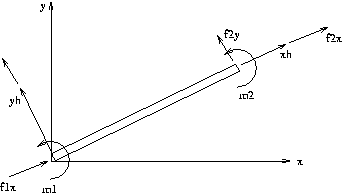
\includegraphics[width=3.0in]{figures/beam}
 \end{center}
 \caption{Sign convention for local forces on a beam element.}
 \label{elements.beam_fig}
\end{figure} 

The three beam type elements ({\tt beam}, {\tt beam3d} and {\tt timoshenko})
all are capable of resolving hinged boundary
conditions for the rotational degrees of freedom.  The adjustment is made
to the element stiffness matrix in global coordinates according to the
following procedure.  Given a hinged DOF, $dof$, then for all entries in 
$k$ (the element stiffness matrix) not associated with $dof$ (all entries
not in row or column $dof$), 
\begin{equation}
k(i,j) = k(i,j) - {k(dof,j) \over k(dof,dof)}k(i,dof).
\end{equation}
The inherent problem in this method of dealing with hinged conditions is
that we cannot calculate any displacements associated with the hinged DOF
and thus, the internal forces calculated for any element with a hinged node 
will not be correct. Displacements other than at the hinged DOF will be
accurate.

\subsubsection{Arbitrarily oriented three-dimensional element}

Like their \mbox{2-d} special case cousins, three-dimensional beam elements are 
two-node linear elements.  \mbox{3-d} beams however, can carry forces in any of the 
six DOFs - axial (local x-direction), vertical shear (local y-direction), 
horizontal shear (local z-direction), rotation about the x-axis (torsion), 
rotation about the y-axis (out-of-plane bending) and rotation about the z-axis 
(in-plane bending).  Both the elastic and shear moduli ({\tt E} and {\tt G}) 
must be specified for a \mbox{3-d} beam element.  The cross-sectional area 
({\tt A}), torsional moment of inertia ({\tt J}), $I_{yy}$ moment of 
inertia ({\tt Iy}) and $I_{zz}$ moment of inertia ({\tt Iz}) must also be 
specified.  {\tt beam3d} elements can define either a lumped or consistent
local mass matrix.  The lumped formulation includes entries at every DOF
(i.e., there is an inertia entry at rotational DOF) just like the 
two-dimensional beam.

The local coordinate system used for the \felt{} \mbox{3-d} beam element is based
on the element geometry presented in \cite{logan:fem}.  Positive
$\hat x$ points from node 1 to node 2.  Then, $\hat y$ is defined by
the cross product of $z$ and $\hat x$ (global z and local x), 
i.e., $\hat y = z \times \hat x$.  $\hat z$ is selected such that it is
orthogonal to the $\hat x$-$\hat y$ plane,  
$\hat z = \hat x \times \hat y$.  Given this geometry, clockwise moments
and rotations about $\hat y$ are positive; for moments and rotations about
$\hat z$, counter-clockwise is defined as positive.

Local internal forces calculated for each \mbox{3-d} beam element include all six
forces at both nodes (twelve total forces for each element).  A distributed 
load on a \mbox{3-d} beam can be directed {\tt parallel} ({\tt LocalX} is 
equivalent) or in the {\tt LocalY},
{\tt LocalZ}, {\tt GlobalX}, {\tt GlobalY}, or {\tt GlobalZ} directions.  
A {\tt parallel} load will be taken as a linearly distributed axial force.  
Like {\tt beam} elements, the sign convention for distributed loads is
based on the appropriate coordinate axes system.
Positive {\tt parallel} loads point from node 1 to node 2.  
Positive loads in the local directions point in the direction of 
of the positive $\hat y$ and $\hat z$ axes, respectively.
The sign conventions 
for loads in the global directions follow the global coordinate axes.  
{\tt beam3d} elements are limited to at most three applied distributed loads.

\subsection{Timoshenko beam element}
\label{elements.timoshenko}
The Timoshenko beam element currently in the library is really intended
as a well-worked example of how to add an element to the \felt{}
system (see Chapter~\ref{adding_elts}).  It is limited to in-plane
behavior and does not support an axial degree of freedom.  

There are lots of approaches to defining an element using Timoshenko
beam theory.  Classic examples can be found in \cite{htk:simple,td:hierarchy}.
The formulation we use is from \cite{kosmatka:timoshenko}.  In all 
formulations, the stiffness matrix is defined as
\begin{equation}
k={EI \over {(1+\phi)L^3}} \left[\matrix{
12 	& 6L		& -12	& 6L \cr
6L	& (4+\phi)L^2	& -6L	& (2-\phi)L^2 \cr
-12	& -6L		& 12	& -6L \cr
6L	& (2-\phi)L^2	& -6L	& (4+\phi)L^2 \cr
}\right].
\end{equation}
In the above equation, $\phi$ is defined as the ratio of the bending
stiffness to shear stiffness,
\begin{equation}
\phi={EI \over {\kappa GA}}.
\end{equation}
$\kappa$ is the shear coefficient from Timoshenko beam theory.  Cowper
\cite{cowper:kappa} provides an approximation for $\kappa$ based
on Poisson's ratio,
\begin{equation}
\kappa={10(1+\nu) \over {12 + 11 \nu}},
\end{equation}
if a better estimate is not available.  This approximation will automatically
be assumed if you provide {\tt nu} rather than {\tt kappa} in the
material property for a Timoshenko beam element.  Because there is no
axial DOF in this formulation, you need to be careful about horizontally
oriented elements; nothing will be assembled into the translational
x DOF in these cases so you should be extra careful about constraints.
The lumped mass matrix for the {\tt timoshenko} element looks just like that
for the 2-d Euler-Bernoulli element (eq.~\ref{beam_lumped}), minus the 
axial DOF of course.  The definition of the consistent mass matrix varies
from one formulation of Timoshenko theory to the next.  The definition in the
formulation that we are using is considerably 
more complicated than the Euler-Bernoulli formulation; 
see~\cite{kosmatka:timoshenko} for details.  

Distributed loads on {\tt timoshenko} elements can only be directed in the
{\tt perpendicular} (equivalent to {\tt LocalY}) direction.  (There are
no axial DOF after all).  The sign conventions for these loads and for
internal forces is the same as that for the standard beam element.
The internal forces calculated will be the shear forces and bending moment at 
each end.

\subsection{Constant Strain Triangular (CST) elements}
\label{elements.cst}

Two different CST elements are in the \felt{} library - one for plane stress  
analysis and one for plane strain analysis.  This means that the only 
difference between the two is that the constitutive matrix, $D$, used in the element 
stiffness formulation is different for the two cases.  A CST element is a 
three-node, two-dimensional, planar element.  Each CST element should exist 
completely in a single x-y plane.  The node numbers must be assigned to a CST 
element in counter-clockwise order to avoid the element having a negative 
area.	

The lumped mass matrix for a CST element is formed simply by dividing the mass
of the element equally between the three nodes, i.e.,
\begin{equation}
m_l={\rho A t \over 3} \left[\matrix{
1 & 0 & 0 & 0 & 0 & 0 \cr
0 & 1 & 0 & 0 & 0 & 0 \cr
0 & 0 & 1 & 0 & 0 & 0 \cr
0 & 0 & 0 & 1 & 0 & 0 \cr
0 & 0 & 0 & 0 & 1 & 0 \cr
0 & 0 & 0 & 0 & 0 & 1 \cr
}\right],
\end{equation}
where $A$ is the computed planar area of the element (not the area as defined
by the material property {\tt A=}). There is no consistent mass formulation 
available for the current set of CST elements.  

Six stress quantities are computed for each CST element: $\sigma_x$, $\sigma_y$,
$\tau_{xy}$, $\sigma_1$, $\sigma_2$, $\theta$, where $\sigma_x$, $\sigma_y$,
$\tau_{xy}$, are the stresses in the global coordinate system, $\sigma_1$, 
$\sigma_2$ are the principal streses, and $\theta$ is the orientation of the 
principal stress axis.  A distributed load on a CST element is taken as an 
in-plane surface traction.  Valid directions for loads are 
{\tt GlobalX} and {\tt GlobalY}. The sign convention for 
load magnitude follows the orientation of the global axes.  Loads which are 
perpendicular or parallel to element sides which are not parallel to one of the 
global axes must be broken down into components which are parallel to the axes 
and then specified as two separate loads.

\subsection{Two-dimensional isoparametric elements}
\label{elements.iso}

\subsubsection{General four to nine node element}

Like CST elements, isoparametric elements are available for either 
plane strain or plane stress analysis.  Isoparametric elements are 2-d planar, 
quadrilateral elements with nine nodes.  Any of the last five nodes are 
optional, however and the fourth node can be the third node repeated.  
The numbering convention is shown in Figure~\ref{elements.iso_numbers}.  
If any of nodes \mbox{5 - 9} are left out, 
their place must be filled with a zero in the {\tt nodes=[ \dots ]} 
specification for that element (i.e. you must always specify nine numbers, it 
is simply that 
any or all of the last five might be specified as zero).  None of the first 
four nodes can be zero.  If the fourth and third nodes are the same, then the 
element will be degenerated to a triangle.  In this case nodes \mbox{5 - 9}
must be zero.	

\begin{figure}
 \begin{center}
  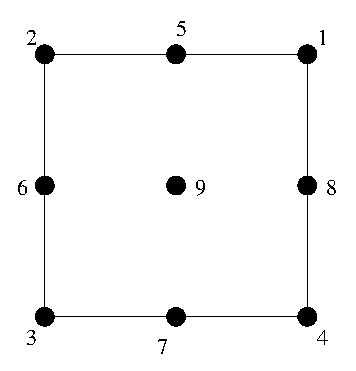
\includegraphics[width=2.5in]{figures/iso_numbers}
 \end{center}
 \caption{Node numbering scheme for nine node isoparametric planar element.}
 \label{elements.iso_numbers}
\end{figure} 

Currently, no stresses are computed for the generalized isoparametric element.
Distributed loads on the generalized isoparametric element are ignored and do 
not affect the problem solution in any way.


\subsubsection{Simple four node element}

{\tt quad\_PlaneStress} and {\tt quad\_PlaneStrain}
elements are just like the generalized 
isoparametric elements described above, but they can only have the first four 
nodes.  They are intended to make problem definition easier in cases where the 
added accuracy that the additional nodes offer is not worth the extra effort.  
Like the generalized case, if the fourth node is the same as the third node 
the element will be degenerated into a triangle.  This allows for easy mixing 
and matching of element shapes without changing element types (though this too 
would be allowed).  	

Distributed loads on the four node isoparametric elements work exactly as 
they do in the CST case.  The stresses computed for each four node 
isoparametric are also the same as those computed for CSTs.  

Like CST elements, only a lumped mass formulation is available for the mass
matrices of isoparametric quadrilateral elements.  The lumped formulation is
generated by lumping the total mass of the element equally at the four nodes
(or the three nodes if the element is being degenerated into a triangle).

\subsection{Plate bending element}
\label{elements.htk}

The plate bending element in \felt{} is a simple four node isoparametric 
quadrilateral that uses selective reduced integration to prevent 
shear locking.  The classic reference for this approach is \cite{htk:simple}.  
The effect is achieved simply by using one-point Gaussian quadrature to 
under-integrate the shear contribution to the stiffness where two-point 
quadrature is used on the bending contributions. 

{\tt htk} elements must exist entirely in the x-y plane; the three DOF
at each node each represent out of plane deformation.  Rotations are
positive in the right-hand sense.  You can generate plate bending triangular 
elements by using {\tt htk} elements with the third and fourth nodes being 
equal (just like you can generate triangles from isoparametric quadrilateral 
elements). Mass matrices for {\tt htk} elements also work the exact same 
way as the mass matrices for the in-plane {\tt quad\_PlaneStress} and
{\tt quad\_PlaneStrain} elements.

Figure~\ref{elements.htk_fig} illustrates the sign convention for the internal
force resultants calculated for each {\tt htk} element.

\begin{figure}
 \begin{center}
  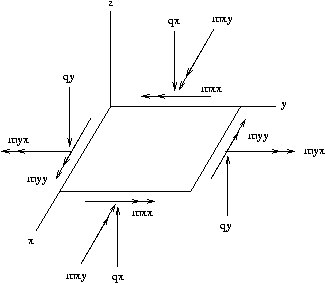
\includegraphics[width=5in]{figures/htk}
 \end{center}
 \caption{Sign convention for force resultants on an htk element.}
 \label{elements.htk_fig}
\end{figure} 

\subsection{Solid brick element}
\label{elements.brick}

The eight-node solid brick element in \felt{} is based on an isoparametric
formulation using linear shape functions.  The element incorporates all
three translational DOF at each node for a total of 24 local degrees of
freedom.  The $24 \times 24$ element stiffness matrix is evaluated using
a fourth-order accurate $2 \times 2 \times 2$ Gaussian quadrature rule.
This formulation results in stress calculations at eight integration points.
Figure~\ref{elements.brick_fig} shows the local node numbering convention
for bricks.  As the figure illustrates, nodes 1-4 and nodes 5-8 must define
opposite faces.
\begin{figure}
 \begin{center}
  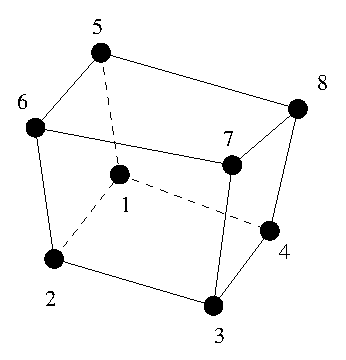
\includegraphics[width=3in]{figures/brick_numbers}
 \end{center}
 \caption{An example of valid node ordering on a brick element.}
 \label{elements.brick_fig}
\end{figure} 

All six independent components of the stress tensor are calculated for brick
elements.  Brick elements are still somewhat limited, however, in that
distributed loads are not handled and element definition routines do
not calculate a mass matrix.  Also, note that because brick elements are the
only solid elements in the \felt{} library, they are also the only elements
which are not fully supported by {\em velvet}, both in terms of problem
definition and in terms of post-processing. 

\subsection{Axisymmetric elements}

The axisymmetric element is a three node triangular element based on
linear shape functions.  The axis of symmetry/revolution is always the 
y-axis.  Distributed loads can be directed in either the {\tt axial} (y)
or {\tt radial} (x) directions.

\section{Thermal analysis elements}

Thermal elements only have one degree of freedom per node,
the nodal temperature.  Prescribed and initial temperatures
are assigned using constraints, {\tt Tx=}, and {\tt iTx=}.
Heat sources are specified using nodal forces ({\tt Fx=}).
For uniform heat sources, simply apply the same force to
all nodes.

\subsection{Rod element}

The rod element is a two node straight line element for thermal
analysis.   Convection surfaces are specified using distributed
loads.  The direction of the load does not matter
and does not need to be specified.  The node, magnitude pairs of
the {\tt values} definition of the load are used to specify the
surface on which the convection is taking place and the convection
coefficient and free stream temperature.  For example
{\tt values=(1,20) (2,50)} specifies a convection coefficient of
20, a free stream temperature of 50, and that the convection acts
over the circumferential surface area of the rod.  If the 
node values are equal in the two pairs then the convecting surface
is taken to be an exposed end of the rod.

\subsection{Constant Temperature Gradient (CTG) element}

The {\tt ctg} element is a thermal analog to the CST triangular
elements for mechanical problems.  
The temperature is assumed to vary linearly over the element.  
As with {\tt rod} elements, convection on {\tt ctg} elements is specified
using distributed loads.  Only the three edges are handled.
The node, magnitude pairs of the {\tt values} definition of the load are 
used to specify the edge on which the convection is taking place and,
as for the rod,  the convection coefficient and free stream temperature.  
For a {\tt ctg element} the definition
{\tt values=(1,20) (2,50)} specifies a convection coefficient of
20, a free stream temperature of 50, and that the convection acts
on the edge defined by local element node numbers 1 and 2.  
